\حصہ{تصور حد کی توسیع}
اس حصے میں ہم حد کی تصور کو وسعت دیتے ہیں۔
\begin{enumerate}[1.]
\item
\ترچھا{یک طرفہ حد۔} جب \عددی{x} نقطہ \عددی{a} تک بائیں ہاتھ سے پہنچنے کی کوشش کرے تب \اصطلاح{بائیں ہاتھ حد}\فرہنگ{حد!بائیں ہاتھ}\حاشیہب{left-handed limit}\فرہنگ{limit!left-handed} حاصل ہو گا۔اسی طرح جب \عددی{x} نقطہ \عددی{a} تک دائیں ہاتھ سے پہنچنے کی کوشش کرے تب \اصطلاح{دائیں ہاتھ حد}\فرہنگ{حد!دائیں ہاتھ}\حاشیہب{right-handed limit}\فرہنگ{limit!right-handed} حاصل ہو گا۔
\item
\ترچھا{لامتناہی حد۔} اگرچہ یہ حقیقی حد نہیں ہے لیکن یہ ان تفاعل کا رویہ بیان کرنے میں مدد دیتی ہے جن کی قیمت بہت زیادہ، مثبت یا منفی، ہو جاتی ہو۔  
\end{enumerate}

\جزوحصہء{یک طرفہ حد}
تفاعل \عددی{f} کا نقطہ \عددی{a} پر حد اص صورت \عددی{L} کے برابر ہو گا جب \عددی{a} کے دونوں اطراف \عددی{f} معین ہو اور \عددی{a} کے دونوں اطراف سے نزدیک تر ہونے کی صورت میں \عددی{f} کی قیمت \عددی{L} کے نزدیک تر پہنچتی ہو۔اسی لئے عام حد کو بعض اوقات \اصطلاح{دو طرفہ حد}\فرہنگ{حد!دو طرفہ}\حاشیہب{two-sided limit}\فرہنگ{limit!two-sided} بھی کہتے ہیں۔

عین ممکن ہے کہ صرف بائیں ہاتھ یا صرف دائیں ہاتھ سے  \عددی{a} کے نزدیک تر ہونے سے \عددی{f} کا حد پایا جاتا ہو۔ایسی صورت میں ہم کہتے ہیں کہ \عددی{f} کا \عددی{a} پر یک طرفہ (بائیں ہاتھ یا دائیں ہاتھ)  حد پایا جاتا ہے۔اگر \عددی{x} نقطہ صفر تک دائیں ہاتھ سے پہنچنے کی کوشش کرے تب تفاعل \عددی{f(x)=\tfrac{x}{\abs{x}}} کا حد \عددی{1} ہو گا جبکہ اگر صفر کو \عددی{x} بائیں ہاتھ سے پہنچنے کی کوششش کرے تب تفاعل کا حد \عددی{-1} ہو گا (شکل \حوالہ{شکل_حد_دایاں_بایاں_مختلف})۔
\begin{figure}
\centering
\begin{minipage}{0.45\textwidth}
\centering
\begin{tikzpicture}
\draw[-latex](-2,0)--(2,0)node[right]{$x$};
\draw[-latex](0,-1.3)--(0,1.5)node[above]{$y$};
\draw(-2,-1)--(0,-1)node[ocirc]{}node[right]{$-1$};
\draw(2,1)--(0,1)node[ocirc]{}node[left]{$1$};
\draw(-1.25,0.75)node[]{$y=\tfrac{x}{\abs{x}}$};
\end{tikzpicture}
\caption{مبدا پر بائیں ہاتھ حد اور دائیں ہاتھ حد مختلف ہیں۔}
\label{شکل_حد_دایاں_بایاں_مختلف}
\end{minipage}\hfill
\begin{minipage}{0.45\textwidth}
\centering
\begin{tikzpicture}
\begin{axis}[axis equal,small,axis lines=middle,xlabel={$x$},ylabel={$y$},xmin=-2.5,xmax=2.5,ymin=-0.2,ymax=2.2,xtick={\empty},ytick={\empty},xlabel style={at={(current axis.right of origin)},anchor=west}]
\addplot[domain=0:180]({2*cos(x)},{2*sin(x)});
\draw(axis cs:-2,0)node[circ]{}node[below]{$-2$} (axis cs:2,0)node[circ]{}node[below]{$2$};
\end{axis}
\end{tikzpicture}
\caption{تفاعل کے دائرہ کار کے آخری سروں پر یک طرفہ حد۔}
\label{شکل_حد_دایاں_بایاں_مختلف_نصف_دائرہ}
\end{minipage}%
\end{figure}

\ابتدا{تعریف}\موٹا{دائیں ہاتھ اور بائیں ہاتھ حد کی غیر رسمی تعریف}\\
فرض کریں کہ وقفہ \عددی{(a,b)}، جہاں \عددی{a<b} ہے ، پر تفاعل \عددی{f(x)} معین ہے۔اگر  اس وقفہ کے اندر سے \عددی{a} تک \عددی{x} پہنچنے کی کوشش کرنے سے \عددی{f(x)} کی قیمت \عددی{L} تک پہنچنے کی کوشش کرتی ہو تب ہم کہتے ہیں کہ \عددی{a} پر \عددی{f(x)} کا \اصطلاح{دائیں ہاتھ حد} \عددی{L} ہے جس کو ہم درج ذیل لکھاتےہیں۔
\begin{align*}
\lim\limits_{x\to a^+} f(x)=L
\end{align*}
فرض کریں کہ وقفہ \عددی{(c,a)}، جہاں \عددی{c<a} ہے ، پر تفاعل \عددی{f(x)} معین ہے۔اگر  اس وقفہ کے اندر سے \عددی{a} تک \عددی{x} پہنچنے کی کوشش کرنے سے \عددی{f(x)} کی قیمت \عددی{M} تک پہنچنے کی کوشش کرتی ہو تب ہم کہتے ہیں کہ \عددی{a} پر \عددی{f(x)} کا \اصطلاح{بائیں ہاتھ حد} \عددی{M} ہے جس کو ہم درج ذیل لکھاتےہیں۔
\begin{align*}
\lim\limits_{x\to a^-} f(x)=M
\end{align*}
شکل \حوالہ{شکل_حد_دایاں_بایاں_مختلف} میں تفاعل \عددی{f(x)=\tfrac{x}{\abs{x}}} کے لئے درج ذیل ہیں۔
\begin{align*}
\lim\limits_{x\to a^+} f(x)=1,\quad \lim\limits_{x\to a^-} f(x)=-1
\end{align*}
\انتہا{تعریف}
%==========================

\عددی{x\to a^+} سے مراد ہے کہ  \عددی{a} تک پہنچتے ہوئے \عددی{x} کی قیمت \عددی{a} سے بڑی رہتی ہے۔ اسی طرح \عددی{x\to a^-} سے مراد ہے کہ  \عددی{a} تک پہنچتے ہوئے \عددی{x} کی قیمت \عددی{a} سے چھوٹی رہتی ہے۔ 

دائرہ کار کے آخری سروں پر تفاعل کا سادہ حد نہیں ہو سکتا ہے البتہ دائرہ کار کے آخری سروں پر تفاعل کا یک طرفہ حد  ہو سکتا ہے۔

\ابتدا{مثال}
تفاعل \عددی{f(x)=\sqrt{4-x^2}} کا دائرہ کار \عددی{[-2,2]} ہے۔تفاعل کی ترسیم نصف دائرہ ہے جس کو شکل \حوالہ{شکل_حد_دایاں_بایاں_مختلف_نصف_دائرہ} میں دکھایا گیا ہے۔دائرہ کار کے آخری سروں پر یک طرفہ حد درج ذیل ہیں۔
\begin{align*}
\lim\limits_{x\to -2^+} \sqrt{4-x^2}=0,\quad  \lim\limits_{x\to 2^-} \sqrt{4-x^2}=0
\end{align*}
نقطہ \عددی{x=-2} پر تفاعل کا بائیں ہاتھ حد نہیں پایا جاتا ہے۔اسی طرح \عددی{x=2} پر اس کا دائیں ہاتھ حد نہیں پایا جاتا ہے۔\عددی{x=-2} اور \عددی{x=2} پر تفاعل کے سادہ دو طرفہ حد نہیں پائے جاتے ہیں۔
\انتہا{مثال}
%=========================

مسئلہ \حوالہ{مسئلہ_حد_قواعد-الف} کے تمام خواص پر یک طرفہ حد پورا اترتا ہے۔دو تفاعل کے مجموعے کا دائیں ہاتھ حد  ان تفاعل  کے انفرادی دائیں ہاتھ حد کا مجموعہ ہو گا، وغیرہ وغیرہ۔کثیر رکنی اور ناطق تفاعل کے حد کے مسئلوں اور مسئلہ بیچ  پر بھی یک طرفہ حد پورا اترتا ہے۔  

یک طرفہ اور دو طرفہ حد کا تعلق درج ذیل مسئلہ پیش کرتا ہے جس کو اس حصے کے آخر میں ثابت  کیا گیا ہے۔

\ابتدا{مسئلہ}\موٹا{یک طرفہ بالمقابل دو طرفہ حد}\\
متغیر \عددی{x} کا \عددی{c} کے نزدیک تر تفاعل \عددی{f(x)} کا حد اس صورت پایا جاتا ہے جب اس نقطے پر تفاعل کا بائیں ہاتھ اور دائیں ہاتھ حد پائے جاتے ہوں اور یہ حد ایک دوسرے کے برابر ہوں:
\begin{align*}
\lim_{x\to c} f(x)=L\quad \Leftrightarrow\quad \lim_{x\to c^-} f(x)=L \quad \text{اور}\quad \lim_{x\to c^+}f(x)=L
\end{align*} 
\انتہا{مسئلہ}
%==========================
\ابتدا{مثال}\شناخت{مثال_حد_یک_طرفہ_دو_طرفہ_الف}
درج ذیل تمام فقرے شکل \حوالہ{شکل_مثال_حد_یک_طرفہ_دو_طرفہ_الف} میں ترسیم شدہ تفاعل کے لئے درست ہیں۔
\begin{description}
\item{\عددی{x=0} پر:}
\عددی{\lim_{x\to 0^+}f(x)=1} ہے جبکہ  \عددی{\lim_{x\to 0^-}f(x)} اور \عددی{\lim_{x\to 0}f(x)} موجود نہیں ہیں۔(\عددی{x=0} کے بائیں جانب تفاعل غیر معین ہے۔)
\item{\عددی{x=1} پر:}
\عددی{\lim_{x\to 1^-}f(x)=0} ہے اگرچہ \عددی{f(1)=1} ہے۔\عددی{\lim_{x\to 1^+}f(x)=1} ہے جبکہ \عددی{\lim_{x\to 1}f(x)} موجود نہیں ہے۔(دائیں ہاتھ اور بائیں ہاتھ حد ایک جیسے نہیں ہیں۔)
\item{\عددی{x=2} پر:}
\عددی{\lim_{x\to 2^-}f(x)=1} اور \عددی{\lim_{x\to 2^+}f(x)=1}  ہیں۔\عددی{\lim_{x\to 2}f(x)=1} ہے اگرچہ \عددی{f(2)=2} ہے۔
\item{\عددی{x=3} پر:}
\عددی{\lim_{x\to 3^-}f(x)=\lim_{x\to 3^+}f(x)=\lim_{x\to 3}f(x)=f(3)=2} ہے۔
\item{\عددی{x=4} پر:}
\عددی{\lim_{x\to 4^-}f(x)=1} ہے اگرچہ \عددی{f(4)\ne 1} ہے۔\عددی{\lim_{x\to 4^+}f(x)} اور \عددی{\lim_{x\to 4}f(x)} موجود نہیں ہیں۔(نقطہ \عددی{x=4} کے دائیں جانب تفاعل غیر معین ہے۔)
\end{description}
اس کے علاوہ \عددی{[0,4]} میں ہر نقطہ \عددی{a} پر  حد \عددی{f(a)} پایا جاتا ہے۔
%
\begin{figure}
\centering
\begin{minipage}{0.45\textwidth}
\centering
\begin{tikzpicture}
\draw[-latex] (-0.25,0)--(5,0)node[right]{$x$};
\draw[-latex](0,-0.2)--(0,2.5)node[above]{$y$};
\foreach \x in {1,2,3,4}{\draw(\x,0)node[below]{$\x$}--++(0,0.1);}
\foreach \y in {1,2}{\draw(0,\y)node[left]{$\y$}--++(0.1,0);}
\draw(0,1)node[circ]{}--(1,0)node[ocirc]{} (1,1)node[circ]{}--(2,1)node[ocirc]{}--(3,2)node[circ]{}--(4,1)node[ocirc]{} (4,0.5)node[circ]{} (2,2)node[circ]{};
\draw(4,1.75)node[right]{$y=f(x)$};
\end{tikzpicture}
\caption{ترسیم برائے مثال \حوالہ{مثال_حد_یک_طرفہ_دو_طرفہ_الف}}
\label{شکل_مثال_حد_یک_طرفہ_دو_طرفہ_الف}
\end{minipage}\hfill
\begin{minipage}{0.45\textwidth}
\centering
\begin{tikzpicture}
\begin{axis}[small,axis lines=middle,xtick={\empty},ytick={-1,1},ymin=-1.2,ymax=1.2,xmax=0.15,xlabel={$x$},ylabel={$y$},ylabel style={at={(current axis.above origin)},anchor=south}]
\addplot[domain=0.02:0.1,samples=200]{sin(deg(1/x))};
\addplot[domain=-0.02:-0.1,samples=200]{sin(deg(1/x))};
\draw(axis cs:0.11,0.8)node[xshift={1mm}]{$y=\sin\tfrac{1}{x}$};
\end{axis}
\end{tikzpicture}
\caption{ترسیم برائے مثال \حوالہ{مثال_حد_یک_طرفہ_دو_طرفہ_ب}}
\label{شکل_مثال_حد_یک_طرفہ_دو_طرفہ_ب}
\end{minipage}%
\end{figure}
\انتہا{مثال}
%==========================

اب تک تمام مثالوں میں جس نقطے پر تفاعل کا حد موجود نہیں تھا وہاں اس کا یک طرفہ حد موجود تھا۔درج ذیل مثال میں ماسوائے نقطہ \عددی{x=0} تفاعل ہر نقطہ پر معین ہے لیکن \عددی{x=0} پر اس کا نہ دائیں ہاتھ اور نا ہی بائیں ہاتھ حد  پایا جاتا ہے۔  

\ابتدا{مثال}\شناخت{مثال_حد_یک_طرفہ_دو_طرفہ_ب}
دکھائیں کہ متغیر \عددی{x} کا دونوں اطراف سے صفر کے نزدیک تر ہونے سے تفاعل  \عددی{y=\sin\tfrac{1}{x}} کا کوئی یک طرفہ حد حاصل نہیں ہوتا ہے (شکل \حوالہ{شکل_مثال_حد_یک_طرفہ_دو_طرفہ_ب})۔\\
حل:\quad
جیسے جیسے \عددی{x}  صفر تک پہنچتا ہے تفاعل \عددی{f(x)=\tfrac{1}{x}} کی قیمت بے قابو بڑھتی ہے جس کی بنا \عددی{\sin\tfrac{1}{x}} کی قیمت متواتر \عددی{-1} اور \عددی{1} کے بیچ تبدیل ہوتی ہے۔ایسا کوئی یکتا عدد \عددی{L} نہیں پایا جاتا ہے جس تک \عددی{\sin\tfrac{1}{x}} کی قیمت قریب تر ہوتی ہو جیسے جیسے \عددی{x} کی (مثبت یا منفی) قیمت صفر کے قریب تر ہوتی جاتی ہے۔یوں \عددی{x=0} پر \عددی{\sin\tfrac{1}{x}} کا نہ کوئی دائیں ہاتھ اور نا کوئی بائیں ہاتھ حد پایا جاتا ہے۔
\انتہا{مثال}
%==========================

\جزوحصہء{لامتناہی حد}
آئیں تفاعل \عددی{f(x)=\tfrac{1}{x}} پر غور کرتے ہیں جس کو گزشتہ مثال میں استعمال کیا گیا ہے۔جیسے جیسے \عددی{x\to 0^+} ہوتا ہے ویسے ویسے تفاعل \عددی{f} کی قیمت بڑھتی ہے حتٰی کہ آخر کار \عددی{f} کی قیمت دیے گئے ہر مثبت حقیقی عدد \عددی{B} سے بڑھ جاتی ہے۔یوں \عددی{B} جتنا بھی بڑا عدد ہو، \عددی{f} آخر کار اس سے بھی بڑا ہو گا (شکل \حوالہ{شکل_حد_قیمت_تجاوز})۔یوں \عددی{x\to 0^+} پر \عددی{f} کا کوئی حد نہیں پایا جاتا ہے۔ اس کے قطع نظر، \عددی{f} کا رویہ بیان کرنے کی خاطر  ہم کہتے ہیں کہ \عددی{x\to 0^+} کرنے سے \عددی{f(x)} کی قیمت \عددی{\infty} کے قریب پہنچتی ہے جس کو درج ذیل لکھا جاتا ہے۔
\begin{align*}
\lim_{x\to 0^+}f(x)=\lim_{x\to 0^+}\frac{1}{x}=\infty
\end{align*}
یہ لکھنے سے ہم ہرگز یہ نہیں کہتے ہیں کہ تفاعل کا حد موجود ہے اور نا ہی ہم کہتے ہیں کہ کوئی حقیقی عدد \عددی{\infty} پایا جاتا ہے چونکہ ایسا کوئی عدد نہیں پایا جاتا ہے۔اس کے برعکس ہم کہتے ہیں کہ \عددی{\lim_{x\to 0^+}\tfrac{1}{x}} موجود نہیں ہے  چونکہ \عددی{x\to 0^+} کرنے سے \عددی{\tfrac{1}{x}} کی قیمت کسی بھی مثبت بڑے عدد سے زیادہ بڑی ہو گی۔

\عددی{x\to 0^-} کرنے سے \عددی{f(x)=\tfrac{1}{x}} کی قیمت کسی بھی منفی بڑی عدد سے زیادہ بڑی منفی ہو گی (یہاں بڑی سے مراد مطلق مقدار ہے)۔یوں \عددی{f(x)} کی قیمت کسی بھی دیے گئے منفی حقیقی عدد \عددی{-B}  سے آخر کار زیادہ منفی ہو گی (شکل \حوالہ{شکل_حد_قیمت_تجاوز})۔ہم درج ذیل لکھتے ہیں۔
\begin{align*}
\lim_{x\to 0^-}f(x)=\lim_{x\to 0^-}\frac{1}{x}=-\infty
\end{align*}
یہاں بھی ہم ہرگز نہیں کہتے ہیں کہ حد موجود ہے اور عدد \عددی{-\infty} کے برابر ہے اور نا ہی کہتے ہیں کہ کوئی حقیقی منفی عدد \عددی{-\infty} پایا جاتا ہے چونکہ ایسا کوئی عدد نہیں پایا جاتا ہے۔ہم اس تفاعل  کا رویہ بیان کرنا چاہتے ہیں جس کی قیمت \عددی{x\to 0^-} کرنے سے کسی بھی بڑی منفی عدد سے زیادہ منفی ہو گی (یہاں بڑی کا لفظ عدد کی مطلق قیمت کے لئے استعمال کیا گیا ہے)۔
\begin{figure}
\centering
\begin{minipage}{0.45\textwidth}
\centering
\begin{tikzpicture}
\begin{axis}[small,axis lines=middle,xlabel={$x$},ylabel={$y$},ytick={\empty},xtick={\empty},ylabel style={at={(current axis.above origin)},anchor=south},xlabel style={at={(current axis.right of origin)},anchor=north}]
\addplot[domain=0.25:3]{1/x}node[pos=0.5,above right]{$y=\frac{1}{x}$};
\addplot[domain=-0.25:-3]{1/x};
\draw(axis cs:0,-3)node[circ]{}node[right]{$-B$};
\draw(axis cs:0,3)node[circ]{}node[left]{$B$};
\end{axis}
\end{tikzpicture}
\caption{تفاعل کی قیمت ہر مثبت یا منفی عدد سے تجاوز کرتی ہے۔}
\label{شکل_حد_قیمت_تجاوز}
\end{minipage}\hfill
\begin{minipage}{0.45\textwidth}
\centering
\begin{tikzpicture}
\begin{axis}[small,axis lines=middle,xlabel={$x$},ylabel={$y$},ytick={-2,-1,1,2},xtick={-2,-1,1,2},ylabel style={at={(current axis.above origin)},anchor=south},xlabel style={at={(current axis.right of origin)},anchor=north}]
\addplot[domain=-2:0.75]{1/(x-1)};
\addplot[domain=1.25:4]{1/(x-1)}node[pos=0.5,above right]{$y=\frac{1}{x-1}$};
\addplot[dashed] plot coordinates {(1,-4) (1,4)};
\end{axis}
\end{tikzpicture}
\caption{ترسیم برائے مثال \حوالہ{مثال_حد_ترسیمی_تحلیلی_حل_الف}}
\label{شکل_مثال_حد_ترسیمی_تحلیلی_حل_الف}
\end{minipage}%
\end{figure}

\ابتدا{مثال}\شناخت{مثال_حد_ترسیمی_تحلیلی_حل_الف}\ترچھا{یک طرفہ حد}\\
\عددی{\lim_{x\to 1^+}\tfrac{1}{x-1}} اور \عددی{\lim_{x\to 1^-}\tfrac{1}{x-1}}  حاصل کریں۔\\
حل:\quad
\موٹا{ترسیمی حل:} تفاعل \عددی{y=\tfrac{1}{x}} کے ترسیم کو \عددی{1} اکائی دائیں منتقل کرنے سے \عددی{y=\tfrac{1}{x-1}} کی ترسیم حاصل ہوتی ہے (شکل \حوالہ{شکل_مثال_حد_ترسیمی_تحلیلی_حل_الف})۔یوں \عددی{1} کے قریب \عددی{y=\tfrac{1}{x-1}} کا رویہ \عددی{0} کے قریب \عددی{y=\tfrac{1}{x}} کے رویہ کی طرح ہو گا۔یوں درج ذیل ہوں گے۔
\begin{align*}
\lim_{x\to 1^+}\frac{1}{x-1}=\infty,\quad\lim_{x\to 1^-}\frac{1}{x-1}=-\infty
\end{align*}
\موٹا{تحلیلی حل:} عدد \عددی{x-1} اور اس کے بالعکس متناسب  پر غور کریں۔\عددی{x\to 1^+} کرنے سے \عددی{(x-1)\to 0^+} اور \عددی{\tfrac{1}{x-1}\to \infty} ملتے ہیں۔\عددی{x\to 1^-} کرنے سے \عددی{(x-1)\to 0^-} اور \عددی{\tfrac{1}{x-1}\to -\infty} ملتے ہیں۔
\انتہا{مثال}
%=======================
\ابتدا{مثال}\شناخت{مثال_حد_ترسیمی_تحلیلی_حل_ب}\ترچھا{دو طرفہ لامتناہی حد}\\
(ا)\quad 
\عددی{x=0} کے قریب \عددی{f(x)=\tfrac{1}{x^2}} (ب) \عددی{x=-3} کے قریب \عددی{g(x)=\tfrac{1}{(x+3)^2}} پر غور کریں۔\\
حل: \quad (ا) جیسے \عددی{x} صفر کو کسی بھی طرف سے پہنچنے کی کوشش کرتا ہے، \عددی{\tfrac{1}{x^2}} کی قیمت مثبت رہتی ہے اور کسی بھی دیے گئے بڑے سے بڑے مثبت عدد \عددی{B}  سے تجاوز کرتی ہے (شکل \حوالہ{شکل_مثال_حد_ترسیمی_تحلیلی_حل_ب}):
\begin{align*}
\lim_{x\to 0}f(x)=\lim_{x\to 0}\frac{1}{x^2}=\infty
\end{align*}
(ب) \عددی{f(x)=\tfrac{1}{x^2}} کی ترسیم کو \عددی{3} اکائیاں بائیں منتقل کرنے سے \عددی{g(x)=\tfrac{1}{(x+3)^2}} کی ترسیم حاصل ہوتا ہے (شکل \حوالہ{شکل_مثال_حد_ترسیمی_تحلیلی_حل_پ})۔یوں \عددی{-3} کے قریب \عددی{g(x)} کا رویہ  \عددی{0} کے قریب \عددی{f(x)} کے رویہ کی طرح ہو گا۔
\begin{align*}
\lim_{x\to -3}g(x)=\lim_{x\to -3}\frac{1}{(x+3)^2}=\infty
\end{align*}
%
\begin{figure}
\centering
\begin{minipage}{0.45\textwidth}
\centering
\begin{tikzpicture}
\begin{axis}[small,axis lines=middle,xlabel={$x$},ylabel={$y$},ytick={\empty},xtick={\empty},ylabel style={at={(current axis.above origin)},anchor=south},xlabel style={at={(current axis.right of origin)},anchor=north},ymin=0]
\addplot[domain=0.5:3]{1/x^2}node[pos=0.5,above right]{$y=\frac{1}{x^2}$};
\addplot[domain=-0.5:-3]{1/x^2};
\draw(axis cs:0,3)node[circ]{}node[left]{$B$};
\end{axis}
\end{tikzpicture}
\caption{تفاعل \عددی{f(x)=\tfrac{1}{x^2}} کی ترسیم (مثال \حوالہ{مثال_حد_ترسیمی_تحلیلی_حل_ب})}
\label{شکل_مثال_حد_ترسیمی_تحلیلی_حل_ب}
\end{minipage}\hfill
\begin{minipage}{0.45\textwidth}
\centering
\begin{tikzpicture}
\begin{axis}[small,axis lines=middle,xlabel={$x$},ylabel={$y$},ytick={\empty},xtick={-3},ylabel style={at={(current axis.above origin)},anchor=south},xlabel style={at={(current axis.right of origin)},anchor=north},xmax=0.5]
\addplot[domain=-3.5:-6]{1/((x+3)^2)};
\addplot[domain=-2.5:0.2]{1/((x+3)^2)}node[pos=0.3,above right]{$y=\frac{1}{(x+3)^2}$};
\addplot[dashed] plot coordinates {(-3,0) (-3,4)};
\end{axis}
\end{tikzpicture}
\caption{تفاعل \عددی{g(x)=\tfrac{1}{(x+3)^2}} کی ترسیم (مثال \حوالہ{مثال_حد_ترسیمی_تحلیلی_حل_ب})}
\label{شکل_مثال_حد_ترسیمی_تحلیلی_حل_پ}
\end{minipage}%
\end{figure}
\انتہا{مثال}
%========================

\عددی{x\to 0} کرنے سے تفاعل \عددی{y=\tfrac{1}{x}} کا رویہ ثابت قدم نہیں رہتا ہے۔ \عددی{x\to 0^+} کرنے سے \عددی{\tfrac{1}{x}\to \infty} حاصل ہوتا ہے جبکہ \عددی{x\to 0^-} کرنے سے \عددی{\tfrac{1}{x} \to -\infty} حاصل ہوتا ہے۔یوں ہم صرف اتنا کہہ سکتے ہیں کہ \عددی{\lim_{x\to 0}\tfrac{1}{x}} موجود نہیں ہے۔ اس کے برعکس تفاعل \عددی{y=\tfrac{1}{x^2}} کا رویہ ثابت قدم ہے۔صفر کے دونوں اطراف سے \عددی{x} کو قریب لانے سے \عددی{\tfrac{1}{x^2}\to \infty} حاصل ہوتا ہے لہٰذا ہم کہتے ہیں کہ \عددی{\lim_{x\to 0}\tfrac{1}{x^2}=\infty} ہے۔

\ابتدا{مثال}\ترچھا{ناطق تفاعل کے نسب نما کے صفر کے قریب تفاعل کے مختلف رویہ دیکھنے کو ملتے ہیں}\\
\begin{align*}
\lim_{x\to 2}\frac{(x-2)^2}{x^2-4}&=\lim_{x\to 2} \frac{(x-2)^2}{(x-2)(x+2)}=\lim_{x\to 2}\frac{x-2}{x+2}=0 && \text{(ا)}\\
\lim_{x\to 2}\frac{x-2}{x^2-4}&=\lim_{x\to 2} \frac{x-2}{(x-2)(x+2)}=\lim_{x\to 2}\frac{1}{x+2}=\frac{1}{4}&& \text{(ب)}\\
\lim_{x\to 2^+}\frac{x-3}{x^2-4}&=\lim_{x\to 2^+} \frac{x-3}{(x-2)(x+2)}=-\infty&& \text{(ج)}\\
\lim_{x\to 2^-}\frac{x-3}{x^2-4}&=\lim_{x\to 2^-} \frac{x-3}{(x-2)(x+2)}=\infty&& \text{(د)}\\
\lim_{x\to 2}\frac{x-3}{x^2-4}&=\lim_{x\to 2} \frac{x-3}{(x-2)(x+2)} \,\,\text{\RL{موجود نہیں}}&& \text{(و)}\\
\lim_{x\to 2}\frac{2-x}{(x-2)^3}&=\lim_{x\to 2} \frac{-(x-2)}{(x-2)^3}=\lim_{x\to 2}\frac{-1}{(x-2)^2}=-\infty && \text{(ہ)}
\end{align*}
جزو (ا) اور (ب) میں \عددی{x=2} پر نسب نما کا صفر شمار کنندہ کے صفر کے ساتھ کٹ جاتا ہے لہٰذا غیر متناہی حد پایا جاتا ہے۔جزو (ہ) میں ایسا نہیں ہے جہاں کٹنے کے بعد بھی نسب نما میں صفر  باقی رہتے ہیں۔
\انتہا{مثال}
%===========================

\جزوحصہء{یک طرفہ حد کی با ضابطہ تعریف}
دو طرفہ حد کی با ضابطہ تعریف کو تبدیل کرتے ہوئے یک طرفہ حد کی تعریف حاصل کی جا سکتی ہے۔

\ابتدا{تعریف}
\موٹا{دائیں ہاتھ حد}\\
اگر ہر عدد \عددی{\epsilon>0} کے لئے ایسا مطابقتی عدد \عددی{\delta>0} پایا جاتا ہو کہ \عددی{x_0<x<x_0+\delta} میں  تمام \عددی{x} کے لئے
\begin{align}\label{مساوات_حد_دائیں_ہاتھ_حد}
x_0<x<x_0+\delta\quad \implies \quad \abs{f(x)-L}<\epsilon
\end{align}
ہو تب ہم کہتے ہیں کہ کہ \عددی{f(x)} کا دائیں ہاتھ حد \عددی{L} ہے۔اس کو درج ذیل لکھا جاتا ہے  (شکل \حوالہ{شکل_حد_دائیں_ہاتھ_تعریف})۔
\begin{align*}
\lim_{x\to x_0^+} f(x)=L &&
\end{align*}
\موٹا{بائیں ہاتھ حد}\\
اگر ہر عدد \عددی{\epsilon>0} کے لئے ایسا مطابقتی عدد \عددی{\delta>0} پایا جاتا ہو کہ \عددی{x_0-\delta<x<x_0} میں  تمام \عددی{x} کے لئے
\begin{align}\label{مساوات_حد_بائیں_ہاتھ_حد}
x_0-\delta<x<x_0\quad \implies \quad \abs{f(x)-L}<\epsilon
\end{align}
ہو تب ہم کہتے ہیں کہ کہ \عددی{f(x)} کا بائیں ہاتھ حد \عددی{L} ہے۔اس کو درج ذیل لکھا جاتا ہے (شکل \حوالہ{شکل_حد_بائیں_ہاتھ_تعریف})۔
\begin{align*}
\lim_{x\to x_0^-} f(x)=L
\end{align*}
%
\begin{figure}
\centering
\begin{minipage}{0.45\textwidth}
\centering
\begin{tikzpicture}
\draw[-latex](-0.25,0)--(4,0)node[right]{$x$};
\draw[-latex](0,-0.2)--(0,3.2)node[above]{$y$};
%\draw(2,0)node[ocirc]{}node[below]{$x_0$};
\draw(1,0)node[ocirc]{}node[below]{$x_0$};
\draw(3,0)node[]{$)$}node[below]{$x_0+\delta$};
\draw(2.4,0)node[circ]{}node[above]{$x$};
\draw[-latex](1,-0.75)--(3,-0.75)node[pos=0.75,below]{$\delta$};
\draw(0,1.5)node[left]{$L$}--++(0.1,0);
\draw(0,0.5)node[rotate=90]{$($}node[left,xshift={-1mm}]{$L-\epsilon$};
\draw(0,2.5)node[rotate=90]{$)$}node[left,xshift={-1mm}]{$L+\epsilon$};
\draw(0,2.1)node[circ]{}node[right]{$f(x)$};
\draw [decorate,decoration={brace,amplitude=10pt},yshift=10pt](1,0) -- (3,0)node [black,midway,yshift=15pt] {\footnotesize
\RL{یہاں تمام $x\ne x_0$ کے لئے}};
\draw [decorate,decoration={brace,amplitude=10pt},xshift=20pt](0,2.5) -- (0,0.5)node [black,midway,right,xshift=9pt] {\footnotesize
\RL{$f(x)$ یہاں رہے گا}};
\end{tikzpicture}
\caption{دائیں ہاتھ حد کی تعریف}
\label{شکل_حد_دائیں_ہاتھ_تعریف}
\end{minipage}\hfill
\begin{minipage}{0.45\textwidth}
\centering
\begin{tikzpicture}
\draw[-latex](-0.25,0)--(4,0)node[right]{$x$};
\draw[-latex](0,-0.2)--(0,3.2)node[above]{$y$};
%\draw(2,0)node[ocirc]{}node[below]{$x_0$};
\draw(1,0)node[]{$($}node[below]{$x_0-\delta$};
\draw(3,0)node[ocirc]{}node[below]{$x_0$};
\draw(1.75,0)node[circ]{}node[above]{$x$};
\draw[latex-](1,-0.75)--(3,-0.75)node[pos=0.75,below]{$\delta$};
\draw(0,1.5)node[left]{$L$}--++(0.1,0);
\draw(0,0.5)node[rotate=90]{$($}node[left,xshift={-1mm}]{$L-\epsilon$};
\draw(0,2.5)node[rotate=90]{$)$}node[left,xshift={-1mm}]{$L+\epsilon$};
\draw(0,2.1)node[circ]{}node[right]{$f(x)$};
\draw [decorate,decoration={brace,amplitude=10pt},yshift=10pt](1,0) -- (3,0)node [black,midway,yshift=15pt] {\footnotesize
\RL{یہاں تمام $x\ne x_0$ کے لئے}};
\draw [decorate,decoration={brace,amplitude=10pt},xshift=20pt](0,2.5) -- (0,0.5)node [black,midway,right,xshift=9pt] {\footnotesize
\RL{$f(x)$ یہاں رہے گا}};
\end{tikzpicture}
\caption{بائیں ہاتھ حد کی تعریف}
\label{شکل_حد_بائیں_ہاتھ_تعریف}
\end{minipage}%
\end{figure}
\انتہا{تعریف}
%=========================

\جزوحصہء{یک طرفہ اور دو طرفہ حد کا آپس میں تعلق}
مساوات \حوالہ{مساوات_حد_دائیں_ہاتھ_حد} اور مساوات \حوالہ{مساوات_حد_بائیں_ہاتھ_حد} میں \عددی{\delta} عدم مساوات سے \عددی{x_0} منفی کرنے سے یک طرفہ اور دو طرفہ حد کا تعلق حاصل ہوتا ہے۔دائیں ہاتھ حد کے لئے، \عددی{x_0} منفی کرنے سے درج ذیل حاصل ہو گا۔
\begin{align}\label{مساوات_حد_یک_طرفہ_الف}
0<x-x_0<\delta\quad \implies \quad \abs{f(x)-L}<\epsilon
\end{align}
بائیں ہاتھ حد کے لئے  \عددی{x_0} منفی کرنے سے درج ذیل حاصل ہو گا۔
\begin{align}\label{مساوات_حد_یک_طرفہ_ب}
-\delta<x-x_0<0\quad \implies \quad \abs{f(x)-L}<\epsilon
\end{align}
مساوات \حوالہ{مساوات_حد_یک_طرفہ_الف} اور مساوات \حوالہ{مساوات_حد_یک_طرفہ_ب} بھی وہی بات کرتے ہیں جو دو طرفہ حد کے لئے درست ہے یعنی:
\begin{align}\label{مساوات_حد_یک_طرفہ_پ}
0<\abs{x-x_0}<\delta\quad \implies \quad \abs{f(x)-L}<\epsilon
\end{align}
یوں \عددی{x_0} پر \عددی{f} کا حد اس صورت \عددی{L} ہو گا اگر \عددی{x_0} پر \عددی{f} کا بائیں ہاتھ حد \عددی{L}  اور دائیں ہاتھ حد \عددی{L} ہو۔

\جزوحصہء{لامتناہی حد کی با ضابطہ تعریف}
بجائے یہ کہ \عددی{x_0} کے کافی قریب تمام \عددی{x} کے لئے ہم کہیں کہ  \عددی{f(x)} کی قیمت عدد \عددی{L} کے قریب سے قریب تر ہو، لامتناہی حد کی تعریف میں ہم کہتے ہیں کہ مبدا سے  \عددی{f(x)} کا فاصلہ کسی بھی دیے عدد سے زیادہ ہو۔اس کے علاوہ حد کی تعریف میں استعمال ہونے والی زبان میں کوئی فرق نہیں پایا جاتا ہے۔شکل \حوالہ{شکل_حد_لامتناہی_تعریف}  کو دیکھ کر درج ذیل تعریف پڑھیں۔
\begin{figure}
\centering
\begin{minipage}{0.45\textwidth}
\centering
\begin{tikzpicture}
\draw[-latex] (-0.5,0)--(3,0)node[right]{$x$};
\draw[-latex](0,-0.2)--(0,2)node[above]{$y$};
\draw[name path=CA](0.75,2) to [out=-100,in=50](-0.5,-0.2);
\draw[name path=CB](1.25,2)node[right]{$y=f(x)$} to [out=-80,in=135](2,0);
\draw[dashed](1,0)node[below]{$x_0$}--(1,2);
\path[name path=kV](1.5,0)--++(0,2);
\draw[dashed,name intersections={of={CB and kV}}](1.5,0)node[pin=-60:{$x_0+\delta$}]{}--(intersection-1);
\draw[name path=CC,dashed,shorten <=-0.25cm](intersection-1)--($(0,0)!(intersection-1)!(0,2)$)node[left]{$B$};
\path[name path=kV](0.5,0)--++(0,2);
\draw[dashed,name intersections={of={CA and kV}}](0.5,0)node[pin=-120:{$x_0-\delta$}]{}--(intersection-1);
\draw[dashed,name intersections={of={CC and CA}}] (intersection-1)--($(0,0)!(intersection-1)!(3,0)$);
\draw(2,1.25)node[right]{$\lim\limits_{x\to x_0}f(x)=\infty$};
\end{tikzpicture}
\end{minipage}\hfill
\begin{minipage}{0.45\textwidth}
\centering
\begin{tikzpicture}[y=-1cm]
\draw[-latex] (-0.75,0)--(3,0)node[right]{$x$};
\draw[latex-](0,-0.5)node[above]{$y$}--(0,2);
\draw[name path=CA](0.75,2) to [out=100,in=-50](-0.5,0);
\draw[name path=CB](1.25,2)node[right]{$y=f(x)$} to [out=80,in=-135](2,0);
\draw[dashed](1,0)node[above]{$x_0$}--(1,2);
\path[name path=kV](1.5,0)--++(0,2);
\draw[dashed,name intersections={of={CB and kV}}](1.5,0)node[pin=50:{$x_0+\delta$}]{}--(intersection-1);
\draw[name path=CC,dashed,shorten <=-0.25cm](intersection-1)--($(0,0)!(intersection-1)!(0,2)$)node[left]{$-B$};
\path[name path=kV](0.5,0)--++(0,2);
\draw[dashed,name intersections={of={CA and kV}}](0.5,0)node[pin=80:{$x_0-\delta$}]{}--(intersection-1);
\draw[dashed,name intersections={of={CC and CA}}] (intersection-1)--($(0,0)!(intersection-1)!(3,0)$);
\draw(2,1.25)node[right]{$\lim\limits_{x\to x_0}f(x)=-\infty$};
\end{tikzpicture}
\end{minipage}%
\caption{لامتناہی حد کی تعریف}
\label{شکل_حد_لامتناہی_تعریف}
\end{figure}

\ابتدا{تعریف}\موٹا{لامتناہی حد}\\
(ا)\quad
اگر ہر مثبت حقیقی عدد \عددی{B} کے لئے ایسا مطابقتی عدد \عددی{\delta>0} پایا جاتا ہو کہ  \عددی{0<\abs{x-x_0}<\delta} میں تمام \عددی{x} کے لئے \عددی{f(x)>B} ہو تب ہم کہتے ہیں کہ جیسے جیسے \عددی{x} کی قیمت \عددی{x_0} کے نزدیک تر ہوتی جاتی ہے ویسے ویسے \عددی{f(x)} کی قیمت لامتناہی کے نزدیک تر ہوتی جاتی ہے۔اس کو درج ذیل لکھا جاتا ہے۔
\begin{align*}
\lim_{x\to x_0} f(x)=\infty
\end{align*}   
(ب)\quad
اگر ہر منفی حقیقی عدد \عددی{-B} کے لئے ایسا مطابقتی عدد \عددی{\delta>0} پایا جاتا ہو کہ  \عددی{0<\abs{x-x_0}<\delta} میں تمام \عددی{x} کے لئے \عددی{f(x)<-B} ہو تب ہم کہتے ہیں کہ جیسے جیسے \عددی{x} کی قیمت \عددی{x_0} کے نزدیک تر ہوتی جاتی ہے ویسے ویسے \عددی{f(x)} کی قیمت منفی لامتناہی کے نزدیک تر ہوتی جاتی ہے۔اس کو درج ذیل لکھا جاتا ہے۔
\begin{align*}
\lim_{x\to x_0} f(x)=-\infty
\end{align*}  
\انتہا{تعریف}
%========================

یک طرفہ حد کی با ضابطہ تعریف بالکل اسی طرح ہے۔اس تعریف کو سوالات میں پیش کیا گیا ہے۔

\حصہء{سوالات}
\موٹا{حد بذریعہ ترسیم}\\
\ابتدا{سوال}\شناخت{سوال_حد_فقرے_درست_الف}
درج ذیل فقروں میں سے کون سے فقرے شکل \حوالہ{شکل_سوال_حد_فقرے_درست_الف}  میں دیے گئے تفاعل \عددی{y=f(x)} کے لئے درست ہیں۔
\begin{multicols}{2}
\begin{enumerate}[a.]
\item
$\lim\limits_{x\to -1^+} f(x)=1$
\item
$\lim\limits_{x\to 0^-} f(x)=0$
\item
$\lim\limits_{x\to 0^-} f(x)=1$
\item
$\lim\limits_{x\to 0^-} f(x)=\lim\limits_{x\to 0^+}f(x)$
\item
$\lim\limits_{x\to 0} f(x)$ 
موجود ہے۔
\item
$\lim\limits_{x\to 0} f(x)=0$
\item
$\lim\limits_{x\to 0} f(x)=1$
\item
$\lim\limits_{x\to 1} f(x)=1$
\item
$\lim\limits_{x\to 1} f(x)=0$
\item
$\lim\limits_{x\to 2^-} f(x)=2$
\item
$\lim\limits_{x\to -1^-} f(x)$
غیر موجود ہے۔
\item
$\lim\limits_{x\to 2^+} f(x)=0$
\end{enumerate}
\end{multicols}
%
\begin{figure}
\centering
\begin{minipage}{0.45\textwidth}
\centering
\begin{tikzpicture}
\draw[-latex](-1.5,0)--(2.5,0)node[right]{$x$};
\draw[-latex] (0,-0.2)--(0,1.5)node[above]{$y$};
\draw[thick,domain=-1:1] plot (\x,\x*\x);
\draw(0,1)node[circ]{}node[left]{$1$}--++(0.1,0);
\foreach \x in {-1,1,2}{\draw(\x,0)node[below]{$\x$}--++(0,0.1);}
\draw(0,0)node[ocirc]{} (-1,1)node[circ]{} (1,1)node[ocirc]{}; 
\draw[thick] (1,0)node[circ]{}--(2,0)node[circ]{};
\draw(1.5,0.5)node[right]{$y=f(x)$};
\end{tikzpicture}
\caption{تفاعل برائے سوال \حوالہ{سوال_حد_فقرے_درست_الف}}
\label{شکل_سوال_حد_فقرے_درست_الف}
\end{minipage}\hfill
\begin{minipage}{0.45\textwidth}
\centering
\begin{tikzpicture}
\draw[-latex](-1.5,0)--(3.5,0)node[right]{$x$};
\draw[-latex] (0,-0.2)--(0,2.5)node[above]{$y$};
\draw[thick] (-1,1)node[circ]{} to [out=-30,in=130] (0,0) to [out=55,in=-120](1,2)node[ocirc]{};
\draw[thick](1,1)node[circ]{}--(2,1)node[ocirc]{}--(3,1)node[circ]{} (2,2)node[circ]{}; 
\draw(2,2.5)node[]{$y=f(x)$};
\foreach \x in {-1,1,2,3}{\draw(\x,0)node[below]{$\x$}--++(0,0.1);}
\foreach \y in {1,2}{\draw(0,\y)node[left]{$\y$}--++(0.1,0);}
\end{tikzpicture}
\caption{تفاعل برائے سوال \حوالہ{سوال_حد_فقرے_درست_ب}}
\label{شکل_سوال_حد_فقرے_درست_ب}
\end{minipage}%
\end{figure}

\انتہا{سوال}
%=======================
\ابتدا{سوال}\شناخت{سوال_حد_فقرے_درست_ب}
درج ذیل میں سے کون سے فقرے شکل \حوالہ{شکل_سوال_حد_فقرے_درست_ب} میں دیے تفاعل کے لئے درست اور کون سے غلط ہیں۔
\begin{multicols}{2}
\begin{enumerate}[a.]
\item
$\lim\limits_{x\to -1^+}f(x)=1$
\item
$\lim\limits_{x\to 2}f(x)$
غیر موجود ہے۔
\item
$\lim\limits_{x\to 2}f(x)=2$
\item
$\lim\limits_{x\to 1^-}f(x)=2$
\item
$\lim\limits_{x\to 1^+}f(x)=1$
\item
$\lim\limits_{x\to 1}f(x)$
غیر موجود ہے۔
\item
$\lim\limits_{x\to 0^+}f(x)=\lim\limits_{x\to 0^-}f(x)$
\item
کھلے وقفہ \عددی{(-1,1)} میں ہر \عددی{c} پر 
$\lim\limits_{x\to c}f(x)$
موجود ہے۔
\item
کھلے وقفہ \عددی{(1,3)} میں ہر \عددی{c} پر 
$\lim\limits_{x\to c}f(x)$
موجود ہے۔
\item
$\lim\limits_{x\to -1^-}f(x)=0$
\item
$\lim\limits_{x\to 3^+}f(x)$
غیر موجود ہے۔
\end{enumerate}
\end{multicols}
\انتہا{سوال}
%=========================
\ابتدا{سوال}\شناخت{سوال_حد_فقرے_درست_ج}
درج ذیل تفاعل کو شکل \حوالہ{سوال_حد_فقرے_درست_ج} میں ترسیم کیا گیا ہے۔
\begin{align*}
f(x)=\begin{cases} 3-x,&x<2\\ \tfrac{x}{2}+1,&x>2 \end{cases}
\end{align*}
%
\begin{enumerate}[a.]
\item
\عددی{\lim_{x\to 2^+}f(x)} اور \عددی{\lim_{x\to 2^-}f(x)} تلاش کریں۔
\item
کیا \عددی{\lim_{x\to 2}f(x)} موجود ہے؟ اگر ہے تو اس کو تلاش کریں اور اگر نہیں ہے تو نا ہونے کی وجہ پیش کریں۔
\item
\عددی{\lim_{x\to 4^-}f(x)} اور \عددی{\lim_{x\to 4^+}f(x)} تلاش کریں۔
\item
کیا \عددی{\lim_{x\to 4}f(x)} موجود ہے۔اگر موجود ہے تو اس کو تلاش کریں اور اگر نہیں ہے تا نا ہونے کی وجہ پیش کریں۔
\end{enumerate}
%
\begin{figure}
\centering
\begin{minipage}{0.45\textwidth}
\centering
\begin{tikzpicture}
\begin{axis}[height=3cm,small,axis lines=middle,ymin=-0.2,xlabel={$x$},ylabel={$y$}]
\addplot[domain=-0.5:2]{3-x}node[pos=0.4,pin=60:{$y=3-x$}]{};
\addplot[domain=2:7]{x/2+1}node[pos=0.4,below right]{$y=\tfrac{x}{2}+1$};
\draw(axis cs:2,1)node[ocirc]{};
\draw(axis cs:2,2)node[ocirc]{};
\end{axis}
\end{tikzpicture}
\caption{تفاعل برائے سوال \حوالہ{سوال_حد_فقرے_درست_ج}}
\label{شکل_سوال_حد_فقرے_درست_ج}
\end{minipage}\hfill
\begin{minipage}{0.45\textwidth}
\centering
\begin{tikzpicture}
\begin{axis}[height=3cm,small,axis lines=middle,ymin=-0.2,xlabel={$x$},ylabel={$y$}]
\addplot[domain=-0.5:2]{3-x}node[pos=0.4,pin=60:{$y=3-x$}]{};
\addplot[domain=2:4]{x/2}node[pos=0.4,below right]{$y=\tfrac{x}{2}$};
\draw(axis cs:2,1)node[ocirc]{};
\draw(axis cs:2,2)node[circ]{};
\end{axis}
\end{tikzpicture}
\caption{تفاعل برائے سوال \حوالہ{سوال_حد_فقرے_درست_چ}}
\label{شکل_سوال_حد_فقرے_درست_چ}
\end{minipage}%
\end{figure}
\انتہا{سوال}
%========================
\ابتدا{سوال}\شناخت{سوال_حد_فقرے_درست_چ}
درج ذیل کو شکل \حوالہ{شکل_سوال_حد_فقرے_درست_چ} میں ترسیم کیا گیا ہے۔
\begin{align*}
f(x)=\begin{cases}
3-x,&x<2\\
2,&x=2\\
\frac{x}{2},&x>2
\end{cases}
\end{align*}
%
\begin{enumerate}[a.]
\item
\عددی{\lim\limits_{x\to 2^+}f(x)}، \عددی{\lim\limits_{x\to 2^-}f(x)} اور \عددی{f(2)} تلاش کریں۔
\item
کیا \عددی{\lim\limits_{x\to 2}f(x)} موجود ہے؟ اگر ہے تو اس کو تلاش کریں۔اگر نہیں ہے تب نا ہونے کی وجہ پیش کریں۔
\item
\عددی{\lim\limits_{x\to -1^-}f(x)} اور \عددی{\lim\limits_{x\to -1^+}f(x)} تلاش کریں۔
\item
کیا \عددی{\lim\limits_{x\to -1}f(x)} موجود ہے؟ اگر ہے تو اس کو تلاش کریں۔اگر نہیں ہے تب نا ہونے کی وجہ پیش کریں۔
\end{enumerate}
\انتہا{سوال}
%=============================
\ابتدا{سوال}\شناخت{سوال_حد_فقرے_درست_ح}
درج ذیل تفاعل کو شکل \حوالہ{شکل_سوال_حد_فقرے_درست_ح} میں ترسیم کیا گیا ہے۔
\begin{align*}
g(x)=\sqrt{x}\sin\frac{1}{x}
\end{align*}
%
\begin{enumerate}[a.]
\item
کیا \عددی{\lim_{x\to 0^+}f(x)} موجود ہے؟ اگر موجود ہے تو اس کو تلاش کریں اور اگر غیر موجود ہے تو غیر موجودگی ہونے کی وجہ پیش کریں۔
\item
کیا \عددی{\lim_{x\to 0^-}f(x)} موجود ہے؟ اگر موجود ہے تو اس کو تلاش کریں اور اگر غیر موجود ہے تو غیر موجودگی ہونے کی وجہ پیش کریں۔
\item
کیا \عددی{\lim_{x\to 0}f(x)} موجود ہے؟ اگر موجود ہے تو اس کو تلاش کریں اور اگر غیر موجود ہے تو غیر موجودگی ہونے کی وجہ پیش کریں۔
\end{enumerate}
%
\begin{figure}
\centering
\begin{minipage}{0.45\textwidth}
\centering
\begin{tikzpicture}
\begin{axis}[clip=false,height=3cm,small,axis lines=middle,xlabel={$x$},ylabel={$y$},xmin=0,ymin=-1.2,ymax=1.5,xtick={\empty},ytick={-1,1}]
\addplot[domain=0.01:0.02,samples=200]{sin(deg(1/x))};
\addplot[domain=0.02:0.06,samples=200]{sin(deg(1/x))};
\draw(axis cs:0,0)node[circ]{};
\draw(axis cs:0.01,1)node[above right]{$y=\begin{cases}0,&x\le 0\\ \sin\tfrac{1}{x},&x>0  \end{cases}$};
\end{axis}
\end{tikzpicture}
\caption{تفاعل برائے سوال \حوالہ{سوال_حد_فقرے_درست_ح}}
\label{شکل_سوال_حد_فقرے_درست_ح}
\end{minipage}\hfill
\begin{minipage}{0.45\textwidth}
\centering
\begin{tikzpicture}
\begin{axis}[clip=false,height=3cm,small,axis lines=middle,xlabel={$x$},ylabel={$y$},xtick={0.3182,0.6365,1},xticklabels={$\tfrac{1}{\pi}$,$\tfrac{2}{\pi}$,$1$},ytick={-1,1}]
\addplot[domain=0:0.25]{sqrt(x)};
\addplot[domain=0.25:1.2]{sqrt(x)}node[pos=0.7,above]{$y=\sqrt{x}$};
\addplot[domain=0:0.25]{-sqrt(x)};
\addplot[domain=0.25:1.2]{-sqrt(x)};
\addplot[domain=0.04:0.1,samples=200]{sqrt(x)*sin(deg(1/x))};
\addplot[domain=0.1:0.2,samples=100]{sqrt(x)*sin(deg(1/x))};
\addplot[domain=0.2:1.2,samples=100]{sqrt(x)*sin(deg(1/x))}node[pos=0.7,below right]{$y=\sqrt{x}\sin\tfrac{1}{x}$};
\end{axis}
\end{tikzpicture}
\caption{تفاعل برائے سوال \حوالہ{سوال_حد_فقرے_درست_خ}}
\label{شکل_سوال_حد_فقرے_درست_خ}
\end{minipage}%
\end{figure}
\انتہا{سوال}
%=====================
\ابتدا{سوال}\شناخت{سوال_حد_فقرے_درست_خ}
درج ذیل تفاعل کو شکل \حوالہ{شکل_سوال_حد_فقرے_درست_خ} میں ترسیم کیا گیا ہے۔
\begin{enumerate}[a.]
\item
کیا \عددی{\lim\limits_{x\to 0^+}g(x)} موجود ہے؟ اگر ہے تو اس کو تلاش کریں اور اگر نہیں ہے تو نا ہونے کی وجہ پیش کریں۔
\item
کیا \عددی{\lim\limits_{x\to 0^-}g(x)} موجود ہے؟ اگر ہے تو اس کو تلاش کریں اور اگر نہیں ہے تو نا ہونے کی وجہ پیش کریں۔
\item
کیا \عددی{\lim\limits_{x\to 0}g(x)} موجود ہے؟ اگر ہے تو اس کو تلاش کریں اور اگر نہیں ہے تو نا ہونے کی وجہ پیش کریں۔
\end{enumerate}
\انتہا{سوال}
%==============================
\ابتدا{سوال}
\begin{enumerate}[a.]
\item
تفاعل
$f\,\,(x)=\begin{cases} x^3,&x\ne 1\\ 0,&x=1 \,\,\end{cases}$
کو ترسیم کریں۔
\item
\عددی{\lim_{x\to 1^-}f(x)} اور \عددی{\lim_{x\to 1^+}f(x)} تلاش کریں۔
\item
کیا \عددی{\lim_{x\to 1}f(x)} موجود ہے؟ اگر ہے تو اس کو تلاش کریں اور اگر نہیں ہے تب نا ہونے کی وجہ پیش کریں۔
\end{enumerate}
\انتہا{سوال}
%====================
\ابتدا{سوال}
\begin{enumerate}[a.]
\item
تفاعل
$f\,\,(x)=\begin{cases} 1-x^2,&x\ne 1\\ 2&x=1 \,\,\end{cases}$
کو ترسیم کریں۔
\item
\عددی{\lim_{x\to 1^-}f(x)} اور \عددی{\lim_{x\to 1^+}f(x)} تلاش کریں۔
\item
کیا \عددی{\lim_{x\to 1}f(x)} موجود ہے؟ اگر ہے تو اس کو تلاش کریں اور اگر نہیں ہے تب نا ہونے کی وجہ پیش کریں۔
\end{enumerate}
\انتہا{سوال}
%====================
سوال \حوالہ{سوال_حد_دو_سوال_الف} اور سوال \حوالہ{سوال_حد_دو_سوال_ب} میں دیے گئے تفاعل کو ترسیم کریں اور درج ذیل کے جوابات دیں۔
\begin{enumerate}[a.]
\item
تفاعل \عددی{f} کے دائرہ کار اور سعت کیا ہیں؟
\item
اگر کسی نقطہ \عددی{c} پر \عددی{\lim_{x\to c}f(x)} موجود ہو تب اس نقطہ کو تلاش کریں۔
\item
کس نقطہ پر صرف بائیں ہاتھ حد وجود ہے؟
\item
کس نقطہ پر صرف دائیں ہاتھ حد موجود ہے؟
\end{enumerate}

\ابتدا{سوال}\شناخت{سوال_حد_دو_سوال_الف}
$f(x)=\begin{cases}\sqrt{1-x^2},&0\le x<1\\ 1,&0\le x<2\\ 2,&x=2  \end{cases}$
\انتہا{سوال}
%=====================
\ابتدا{سوال}\شناخت{سوال_حد_دو_سوال_ب}
$f(x)=\begin{cases}x,&-1\le x<0\,\, \text{یا}\,\, 0<x\le 1\\ 1,& x=0\\ 0,&x<-1 \,\,\text{یا}\,\, x>1  \end{cases}$
\انتہا{سوال}
%==================
\موٹا{حد کا تحلیلی حصول:} سوال \حوالہ{سوال_حد_تحلیلی_تلاش_الف} تا سوال \حوالہ{سوال_حد_تحلیلی_تلاش_ب} میں حد تلاش کریں۔

\ابتدا{سوال}\شناخت{سوال_حد_تحلیلی_تلاش_الف}
$\lim\limits_{x\to -0.5^-}\sqrt{\tfrac{x+2}{x+1}}$
\انتہا{سوال}
%=======================
\ابتدا{سوال}
$\lim\limits_{x\to 1^+}\sqrt{\tfrac{x-1}{x+2}}$
\انتہا{سوال}
%=======================
\ابتدا{سوال}
$\lim\limits_{x\to -2^+}(\tfrac{x}{x+1})(\tfrac{2x+5}{x^2+x})$
\انتہا{سوال}
%=======================
\ابتدا{سوال}
$\lim\limits_{x\to 1^-}(\tfrac{1}{x+1})(\tfrac{x+6}{x})(\tfrac{3-x}{7})$
\انتہا{سوال}
%=======================
\ابتدا{سوال}
$\lim\limits_{h\to 0^+}\tfrac{\sqrt{h^2+4h+5}-\sqrt{5}}{h}$
\انتہا{سوال}
%=======================
\ابتدا{سوال}
$\lim\limits_{h\to 0^-}\tfrac{\sqrt{6}-\sqrt{5h^2+11h+6}}{h}$
\انتہا{سوال}
%=======================
\ابتدا{سوال}
(ا)\quad
$\lim\limits_{x\to -2^+}(x+3)\tfrac{\abs{x+2}}{x+2}$\quad
(ب)\quad
$\lim\limits_{x\to -2^-}(x+3)\tfrac{\abs{x+2}}{x+2}$
\انتہا{سوال}
%=======================
\ابتدا{سوال}
(ا)\quad
$\lim\limits_{x\to 1^+}\tfrac{\sqrt{2x}(x-1)}{\abs{x-1}}$\quad
(ب)\quad
$\lim\limits_{x\to 1^-}\tfrac{\sqrt{2x}(x-1)}{\abs{x-1}}$
\انتہا{سوال}
%=======================
\ابتدا{سوال}
(ا)\quad
$\lim\limits_{\theta\to 3^+}\tfrac{\abs{\theta}}{\theta}$\quad
(ب)\quad
$\lim\limits_{\theta\to 3^-}\tfrac{\abs{\theta}}{\theta}$
\انتہا{سوال}
%=======================
\ابتدا{سوال}\شناخت{سوال_حد_تحلیلی_تلاش_ب}
(ا)\quad
$\lim\limits_{t\to 4^+} (t-\abs{t})$\quad
(ب)\quad
$\lim\limits_{t\to 4^-} (t-\abs{t})$
\انتہا{سوال}
%=======================

\موٹا{لامتناہی حد:} سوال \حوالہ{سوال_حد_لامتناہی_الف} تا سوال \حوالہ{سوال_حد_لامتناہی_ب} میں لامتناہی حد تلاش کریں۔

\ابتدا{سوال}\شناخت{سوال_حد_لامتناہی_الف}
$\lim\limits_{x\to 0^+}\tfrac{1}{3x}$
\انتہا{سوال}
%=========================
\ابتدا{سوال}
$\lim\limits_{x\to 0^-}\tfrac{5}{2x}$
\انتہا{سوال}
%=========================
\ابتدا{سوال}
$\lim\limits_{x\to 2^-}\tfrac{3}{x-2}$
\انتہا{سوال}
%=========================
\ابتدا{سوال}
$\lim\limits_{x\to 3^+}\tfrac{1}{x-3}$
\انتہا{سوال}
%=========================
\ابتدا{سوال}
$\lim\limits_{x\to -8^+}\tfrac{2x}{x+8}$
\انتہا{سوال}
%=========================
\ابتدا{سوال}
$\lim\limits_{x\to -5^-}\tfrac{3x}{2x+10}$
\انتہا{سوال}
%=========================
\ابتدا{سوال}
$\lim\limits_{x\to 7}\tfrac{4}{(x-7)^2}$
\انتہا{سوال}
%=========================
\ابتدا{سوال}
$\lim\limits_{x\to 0}\tfrac{-1}{x^2(x+1)^2}$
\انتہا{سوال}
%=========================
\ابتدا{سوال}
(ا)\quad
$\lim\limits_{x\to 0^+}\tfrac{2}{3x^{1/3}}$\quad
(ب)\quad
$\lim\limits_{x\to 0^-}\tfrac{2}{3x^{1/3}}$
\انتہا{سوال}
%=========================
\ابتدا{سوال}
(ا) \quad
$\lim\limits_{x\to 0^+}\tfrac{2}{x^{1/5}}$\quad
(ب)\quad
$\lim\limits_{x\to 0^-}\tfrac{2}{x^{1/5}}$
\انتہا{سوال}
%=========================
\ابتدا{سوال}
$\lim\limits_{x\to 0}\tfrac{4}{x^{2/5}}$
\انتہا{سوال}
%=========================
\ابتدا{سوال}\شناخت{سوال_حد_لامتناہی_ب}
$\lim\limits_{x\to 0}\tfrac{1}{x^{2/3}}$
\انتہا{سوال}
%=========================

سوال \حوالہ{سوال_حد_سادہ_الف} تا سوال \حوالہ{سوال_حد_سادہ_ب} میں حد تلاش کریں۔

\ابتدا{سوال}\شناخت{سوال_حد_سادہ_الف}
$\lim\limits_{x\to (\pi/2)^-}\tan x$
\انتہا{سوال}
%=================
\ابتدا{سوال}
$\lim\limits_{x\to (-\pi/2)^+}\sec x$
\انتہا{سوال}
%==================
\ابتدا{سوال}
$\lim\limits_{\theta\to 0^-}(1+\csc \theta)$
\انتہا{سوال}
%=========================
\ابتدا{سوال}\شناخت{سوال_حد_سادہ_ب}
$\lim\limits_{\theta\to 0} (2-\cot \theta)$
\انتہا{سوال}
%=========================
\موٹا{مزید حساب:} سوال \حوالہ{سوال_حد_مزید_حساب_الف} تا سوال \حوالہ{سوال_حد_مزید_حساب_ب} میں دی گئی  صورت میں حد تلاش کریں۔

\ابتدا{سوال}\شناخت{سوال_حد_مزید_حساب_الف}
$\lim \tfrac{1}{x^2-4}$
\begin{multicols}{4}
\begin{enumerate}[a.]
\item
$x\to 2^+$
\item
$x\to 2^-$
\item
$x\to -2^+$
\item
$x\to -2^-$
\end{enumerate}
\end{multicols}
\انتہا{سوال}
%=================
\ابتدا{سوال}
$\lim\tfrac{x}{x^2-1}$
\begin{multicols}{4}
\begin{enumerate}[a.]
\item
$x\to 1^+$
\item
$x\to 1^-$
\item
$x\to -1^+$
\item
$x\to -1^-$
\end{enumerate}
\end{multicols}
\انتہا{سوال}
%============================
\ابتدا{سوال}
$\lim(\tfrac{x^2}{2}-\tfrac{1}{x})$
\begin{multicols}{4}
\begin{enumerate}[a.]
\item
$x\to 0^+$
\item
$x\to 0^-$
\item
$x\to \sqrt[\leftroot{-2}3]{2}$
\item
$x\to -1$
\end{enumerate}
\end{multicols}
\انتہا{سوال}
%=========================
\ابتدا{سوال}
$\lim\tfrac{x^2-1}{2x+4}$
\begin{multicols}{4}
\begin{enumerate}[a.]
\item
$x\to -2^+$
\item
$x\to -2^-$
\item
$x\to 1^+$
\item
$x\to 0^-$
\end{enumerate}
\end{multicols}
\انتہا{سوال}
%==========================
\ابتدا{سوال}
$\lim\tfrac{x^2-3x+2}{x^3-2x^2}$
\begin{multicols}{4}
\begin{enumerate}[a.]
\item
$x\to 0^+$
\item
$x\to 2^+$
\item
$x\to 2^-$
\item
$x\to 2$
\end{enumerate}
\end{multicols}
\انتہا{سوال}
%==========================
\ابتدا{سوال}\شناخت{سوال_حد_مزید_حساب_ب}
$\lim\tfrac{x^2-3x+2}{x^3-4x}$
\begin{multicols}{4}
\begin{enumerate}[a.]
\item
$x\to 2^+$
\item
$x\to -2^+$
\item
$x\to 0^-$
\item
$x\to 1^+$
\end{enumerate}
\end{multicols}
\انتہا{سوال}
%==========================
سوال \حوالہ{سوال_حد_صورت_الف} تا سوال \حوالہ{سوال_حد_صورت_ب} میں دی گئی صورتوں میں حد تلاش کریں۔

\ابتدا{سوال}\شناخت{سوال_حد_صورت_الف}
$\lim(2-\tfrac{3}{t^{1/3}})$
\begin{multicols}{4}
\begin{enumerate}[a.]
\item
$t\to 0^+$
\item
$t\to 0^-$
\end{enumerate}
\end{multicols}
\انتہا{سوال}
%=======================
\ابتدا{سوال}
$\lim(\tfrac{1}{t^{\,3/5}}+7)$
\begin{multicols}{4}
\begin{enumerate}[a.]
\item
$t\to 0^+$
\item
$t\to 0^-$
\end{enumerate}
\end{multicols}
\انتہا{سوال}
%=====================
\ابتدا{سوال}
$\lim(\tfrac{1}{x^{2/3}}+\tfrac{2}{(x-1)^{2/3}})$
\begin{multicols}{4}
\begin{enumerate}[a.]
\item
$x\to 0^+$
\item
$x\to 0^-$
\item
$x\to 1^+$
\item
$x\to 1^-$
\end{enumerate}
\end{multicols}
\انتہا{سوال}
%=========================
\ابتدا{سوال}\شناخت{سوال_حد_صورت_ب}
$\lim(\tfrac{1}{x^{1/3}}-\tfrac{1}{(x-1)^{4/3}})$
\begin{multicols}{4}
\begin{enumerate}[a.]
\item
$x\to 0^+$
\item
$x\to 0^-$
\item
$x\to 1^+$
\item
$x\to 1^-$
\end{enumerate}
\end{multicols}
\انتہا{سوال}
%===========================
\موٹا{نظریہ اور مثالیں}

\ابتدا{سوال}
اگر \عددی{f} کے دائرہ کار کے اندر آپ کو \عددی{\lim_{x\to a^+}f(x)} اور \عددی{\lim_{x\to a^-}f(x)} معلوم ہو تب کیا آپ \عددی{\lim_{x\to a}f(x)}  کے بارے میں کچھ کہہ سکتے ہیں؟ اپنے جواب کی وجہ پیش کریں۔
\انتہا{سوال}
%==========================
\ابتدا{سوال}
اگر آپ جانتے ہوں کہ \عددی{\lim_{x\to c}f(x)} موجود ہے، کیا آپ  \عددی{\lim_{x\to c^+}f(x)} تلاش کرتے ہوئے اس حد کو تلاش کر سکتے ہیں؟ اپنے جواب کی وجہ پیش کریں۔
\انتہا{سوال}
%==============================
\ابتدا{سوال}
فرض کریں کہ \عددی{f(x)} متغیر \عددی{x} کا طاق تفاعل ہے۔ کیا یہ جانتے ہوئے کہ \عددی{\lim_{x\to 0^+}f(x)=3} ہے، آپ \عددی{\lim_{x\to 0^-}f(x)=3}  کے بارے میں کچھ کہہ سکتے ہیں؟ اپنے جواب کی وجہ پیش کریں۔
\انتہا{سوال}
%============================
\ابتدا{سوال}
فرض کریں کہ \عددی{f(x)} متغیر \عددی{x} کا جفت تفاعل ہے۔اگر \عددی{\lim_{x\to 2^-}f(x)=7} ہو تب کیا \عددی{\lim_{x\to -2^-}f(x)} یا
 \عددی{\lim_{x\to -2^+}f(x)}  کے بارے میں کچھ کہنا ممکن ہے؟ اپنے جواب کی وجہ پیش کریں۔
\انتہا{سوال}
%============================
\موٹا{یک طرفہ حد کی با ضابطہ تعریف}

\ابتدا{سوال}
اگر \عددی{\epsilon>0} ہو تب ایسا وقفہ \عددی{I=(5,5+\delta),\delta>0} تلاش کریں کہ اگر \عددی{x} وقفہ \عددی{I} میں پایا جاتا ہو تب \عددی{\sqrt{x-5}<\epsilon} ہو۔کس حد کی تصدیق کی جا رہی ہے اور اس کی قیمت کیا ہے؟ 
\انتہا{سوال}
%===================
\ابتدا{سوال}
اگر \عددی{\epsilon>0} ہو تب ایسا وقفہ \عددی{I=(4-\delta,4),\delta >0} تلاش کریں کہ اگر \عددی{x} وقفہ \عددی{I} میں پایا جاتا ہو تب \عددی{\sqrt{4-x}<\epsilon} ہو۔کس حد کی تصدیق کی جا رہی ہے اور اس حد کی قیمت کیا ہے؟
\انتہا{سوال}
%=======================
دائیں ہاتھ اور بائیں ہاتھ حد کی تعریف استعمال کرتے ہوئے سوال \حوالہ{سوال_حد_فقرے_الف} اور سوال \حوالہ{سوال_حد_فقرے_ب} میں دیے الجبرائی فقروں کو ثابت کریں۔

\ابتدا{سوال}\شناخت{سوال_حد_فقرے_الف}
$\lim\limits_{x\to 0^-}\tfrac{x}{\abs{x}}=-1$
\انتہا{سوال}
%=====================
\ابتدا{سوال}\شناخت{سوال_حد_فقرے_ب}
$\lim\limits_{x\to 2^+}\tfrac{x-2}{\abs{x-2}}=1$
\انتہا{سوال}
%===========================
\ابتدا{سوال}
(ا) \عددی{\lim_{x\to 400^+}\lfloor x \rfloor} اور (ب) \عددی{\lim_{x\to 400^-}\lfloor x\rfloor} تلاش کریں۔اس کے بعد حد کی تعریف استعمال کرتے ہوئے اپنے جوابات کی تصدیق کریں۔ (ج) گزشتہ دو جزو کے نتائج کو دیکھ کر کیا \عددی{\lim_{x\to 400}\lfloor x\rfloor} کے بارے میں کچھ کہا جا سکتا ہے؟ اپنے جواب کی وجوہات پیش کریں۔
\انتہا{سوال}
%==========================
\ابتدا{سوال}
فرض کریں کہ 
$\,\,f(x)=\begin{cases}x^2\sin\tfrac{1}{x},&x<0\\ \sqrt{x},&x>0  \,\, \end{cases}$
ہے۔ (ا) \عددی{\lim_{x\to 0^+}f(x)} اور (ب) \عددی{\lim_{x\to 0^-}f(x)} تلاش کریں۔اس کے بعد حد کی تعریف استعمال کرتے ہوئے نتائج کی تصدیق کریں۔کیا ان نتائج کو دیکھ کر \عددی{\lim_{x\to 0}f(x)} کے بارے میں کچھ کہا جا سکتا ہے؟ اپنے جواب کی وجوہات  پیش کریں۔
\انتہا{سوال}
%==================

\موٹا{لامتناہی حد کی با ضابطہ تعریف:} سوال \حوالہ{سوال_حد_لامتناہی_تعریف_الف} تا سوال \حوالہ{سوال_حد_لامتناہی_تعریف_ب} میں دیے گئے فقروں کو حد کی با ضابطہ تعریف کی استعمال سے ثابت کریں۔

\ابتدا{سوال}\شناخت{سوال_حد_لامتناہی_تعریف_الف}
$\lim\limits_{x\to 0}\tfrac{1}{x^2}=\infty$
\انتہا{سوال}
%=======================
\ابتدا{سوال}
$\lim\limits_{x\to 0}\tfrac{-1}{x^2}=-\infty$
\انتہا{سوال}
%===========================
\ابتدا{سوال}
$\lim\limits_{x\to 3}\tfrac{-2}{(x+3)^2}=-\infty$
\انتہا{سوال}
%=========================
\ابتدا{سوال}\شناخت{سوال_حد_لامتناہی_تعریف_ب}
$\lim\limits_{x\to -5}\tfrac{1}{(x+5)^2}=\infty$
\انتہا{سوال}
%=========================
\موٹا{یک طرفہ لامتناہی حد کی با ضابطہ تعریف}

دائیں ہاتھ لا متناہی حد کی تعریف درج ذیل ہے۔

\ابتدا{تعریف}
اگر ہر مثبت حقیقی عدد \عددی{B} کے لئے ایسا مطابقتی عدد \عددی{\delta>0} موجود ہو کہ \عددی{x_0<x<x_0+\delta} میں تمام \عددی{x} کے لئے \عددی{f(x)>B} ہو تب ہم کہتے ہیں کہ جیسے جیسے \عددی{x} دائیں ہاتھ سے \عددی{x_0}  کے نزدیک تر ہوتا جاتا ہے ویسے ویسے \عددی{f(x)} لامتناہی کے نزدیک تر ہوتا جاتا ہے، جس کو ہم درج ذیل لکھتے ہیں۔
\begin{align*}
\lim_{x\to x_0^+}=\infty
\end{align*}
\انتہا{تعریف}
%=========================

\ابتدا{سوال}
درج بالا تعریف کو تبدیل کرتے ہوئے درج ذیل صورتوں کے لئے قابل استعمال بنائیں۔
\begin{multicols}{2}
\begin{enumerate}[a.]
\item
$\lim_{x\to x_0^-}f(x)=\infty$
\item
$\lim_{x\to x_0^+}f(x)=-\infty$
\item
$\lim_{x\to x_0^-}f(x)=-\infty$
\end{enumerate}
\end{multicols}
\انتہا{سوال}
%==================

یک طرفہ لامتناہی حد کی با ضابطہ تعریف استعمال کرتے ہوئے سوال \حوالہ{سوال_حد_تعریف_استعمال_تلاش_الف} تا سوال \حوالہ{سوال_حد_تعریف_استعمال_تلاش_ب} میں دیے گئے فقروں کو ثابت کریں۔ 

\ابتدا{سوال}\شناخت{سوال_حد_تعریف_استعمال_تلاش_الف}
$\lim_{x\to 0^+}\tfrac{1}{x}=\infty$
\انتہا{سوال}
%======================
\ابتدا{سوال}
$\lim_{x\to 0^-}\tfrac{1}{x}=-\infty$
\انتہا{سوال}
%======================
\ابتدا{سوال}
$\lim_{x\to 2^-}\tfrac{1}{x-2}=-\infty$
\انتہا{سوال}
%==========================
\ابتدا{سوال}
$\lim_{x\to 2^+}\tfrac{1}{x-2}=\infty$
\انتہا{سوال}
%==========================
\ابتدا{سوال}
$\lim_{x\to 1^+}\tfrac{1}{1-x^2}=-\infty$
\انتہا{سوال}
%==========================
\ابتدا{سوال}\شناخت{سوال_حد_تعریف_استعمال_تلاش_ب}
$\lim_{x\to 1^-}\tfrac{1}{1-x^2}=\infty$
\انتہا{سوال}
%==========================

\حصہ{استمرار}


